\documentclass[review]{elsarticle}
\usepackage{amsmath,amssymb,booktabs,graphicx}
\usepackage[hidelinks]{hyperref}
\graphicspath{{figs/}}
\newcommand{\own}{p_{\mathrm{own}}}

\journal{Neural Networks}

\begin{document}
\begin{frontmatter}

\title{Repair Headroom, Not Dying Gates:\\
When an Own-Segment Bias Helps Continual Learning\\
--- and When It Silently Reverses}

\author[inst1]{Ranxi Zhou}
\affiliation[inst1]{organization={Independent researcher},
            city={Changsha},
            country={China}}

\begin{abstract}
A recent audit of dendritic context-gated protection (companion paper,
S1) found that a one-hidden-layer active-dendrite network with
winner-take-all routing fails to develop segment--task specialization,
that the standard dominant-segment instrument is contaminated by dead
neurons, and that a constant bias $b$ on the own-segment dendritic
input repairs the learning term ($\Delta\ell$ up to $+4.6$ at
$T{=}20$, $t \ge 8$). We test whether these findings transfer beyond
the bare-MLP family. \textbf{They do not --- and the failure mode is
informative.} On a convolutional active-dendrite network
(4-layer conv trunk + GroupNorm + global average pooling feeding the
identical dendritic gate; $160$ runs, $10$ seeds per cell), the
repair collapses to noise ($\Delta\ell$ significant in $4/12$ dose
cells; largest effect $+1.46$ vs.\ the MLP's $+0.8$ to $+4.6$) and
\emph{final accuracy reverses} ($\Delta\mathrm{avg}$ down to $-2.29$,
$t{=}-3.1$). The dead-neuron artifact disappears entirely --- not
because the instrument improved, but because conv+GroupNorm mortality
is exactly zero where the bare MLP's was $57\%$. A decisive
same-architecture control (GroupNorm inserted into the MLP's feature
layer, $80$ runs, the only delta) separates the two candidate
explanations: mortality and repair-gain \emph{decouple} (GroupNorm
raises mortality to $76.5\%$/$85.5\%$ while collapsing the gain to
$17\%$/$26\%$ of its bare-MLP value), so dying gates are not the
mediating variable; instead, gain decays as the unbiased baseline
strengthens, and on both strong-feature backbones the repair buys
learning only while significantly worsening retention. We conclude
with a practitioner-facing boundary: own-segment bias repairs pay
when the baseline is weak and its gates die; on strong-feature
backbones they silently trade retention for learning, and the
dominant-segment diagnostic must be paired with a mortality probe
before it is trusted anywhere.
\end{abstract}

\begin{keyword}
continual learning \sep dendritic computation \sep active dendrites \sep
reproducibility \sep negative results
\end{keyword}

\end{frontmatter}

% =====================================================================
\section{Introduction}
\label{sec:intro}

Companion paper S1 \cite{zhou2026delpS1} established, on a
one-hidden-layer active-dendrite network (ADNet
\cite{iyer2022}) with $k$-winners-take-all routing, a three-link chain:
(1) the network fails to develop segment--task specialization;
(2) the standard dominant-segment instrument overstates this failure
because dead neurons fall to segment~0 by argmax convention;
(3) a constant bias $b$ on the own-segment dendritic input causally
repairs the learning term with a clean dose--response
($22/22$ dose cells positive, $20/22$ significant at $T \le 20$).

S1's own limitations section asks the question this paper answers:
\emph{does the chain transfer beyond the bare-MLP family?} The question
matters because the repair is deliberately architecture-agnostic ---
a scalar added to one gate --- and because the artifact mechanism
(argmax over dead gates) should exist wherever segments and hard
routing coexist \cite{boahen2022,poirazi2020}.

We test transfer with the same instrument stack and pre-registered
criteria, on two new configurations:

\begin{itemize}
\item \textbf{ConvADNet} --- a 4-layer convolutional trunk with
GroupNorm and global average pooling feeding the \emph{identical}
dendritic gate, kWTA sparsifier, and protected-gradient scheme
($160$ runs; Sec.~\ref{sec:conv});
\item \textbf{GN-MLP} --- the original single-hidden-layer network
with one GroupNorm layer inserted between the feature projection and
the dendritic gate ($80$ runs; Sec.~\ref{sec:gnmlp}). This is a
same-architecture control: every hyperparameter, the routing
structure, and the protection mechanism are unchanged; the norm layer
alone differs.
\end{itemize}

Both transfer attempts fail their pre-registered criteria, and the
\emph{pattern} of failure identifies what the repair actually needs.
The conv network has exactly zero neuronal mortality --- the artifact
vanishes not because the instrument got better but because the
pathology it measures is absent --- and the repair collapses with it.
The GroupNorm control then kills the natural ``dying-gate'' hypothesis:
normalization \emph{raises} mortality while \emph{collapsing} the
repair gain, so the two are decoupled. What tracks the gain instead is
the strength of the unbiased baseline: where the baseline is strong
(GroupNorm, convolution), there is little learning-term room to buy,
and the price shifts entirely to retention --- final accuracy
reverses significantly on both strong-feature configurations
($-3.88$ and $-6.55$ on GN-MLP; $-0.84$ and $-2.29$ on ConvADNet).

\paragraph{Contributions.}
\begin{enumerate}
\item A pre-registered, $160$-run transfer test of the S1 repair to a
convolutional active-dendrite network: the repair does not transfer
($4/12$ cells significant vs.\ $15/20$ required) and final accuracy
reverses (Sec.~\ref{sec:conv}).
\item A zero-mortality finding: conv+GroupNorm keeps every gate
alive, so the dominant-segment artifact of S1 is architecture-bound,
not instrument-bound (Sec.~\ref{sec:conv}).
\item A decisive same-architecture control ($80$ runs, one delta)
showing mortality and repair-gain decouple: the ``dying-gate''
hypothesis is false, and baseline strength --- not gate death --- is
the tracking variable (Sec.~\ref{sec:gnmlp}).
\item A practitioner boundary condition: own-segment bias repairs pay
only on weak-baseline, high-mortality configurations; on
strong-feature backbones they silently trade retention for learning
(Sec.~\ref{sec:discussion}).
\end{enumerate}

All experiments are pre-registered (criteria fixed before data
collection), paired by seed, and reported with all cells --- including
those that failed.

% =====================================================================
\section{Background: the S1 chain being tested}
\label{sec:background}

We summarise only what the transfer test requires; full protocol in
S1 \cite{zhou2026delpS1}. The model is an active-dendrite network
\cite{iyer2022}: features $t = \mathrm{ff}(x)$, a context-conditioned
gate $u = W_d\,\mathrm{ctx}$ reshaped to $(n_{\mathrm{seg}}, n_h)$, a
winning segment per neuron $d = \max_{\mathrm{seg}} u$, hidden
activity $h = \mathrm{kWTA}(t \odot \sigma(d))$ with $k{=}64$, and a
linear readout. Gradients of the gate are protected: only the current
task's segment trains. Protection is usage-localized EWC
\cite{kirkpatrick2017} on the
feature and readout blocks ($\lambda{=}1000$); the protected-gradient
and context-gating design follows \cite{iyer2022,masse2018}. Tasks are
Permuted-MNIST and Permuted-Fashion \cite{parisi2019} at $T \in \{10, 20\}$.

The S1 findings under test:

\begin{enumerate}
\item \textbf{Anti-specialization.} The own-segment win rate stays at
chance ($1/T$) throughout training.
\item \textbf{Dead-neuron artifact.} The naive win rate (all neurons)
is inflated $0.62$ vs.\ $0.11$ (active) by argmax ties over dead
gates; mortality at $T{=}10$ is $57.2\%$.
\item \textbf{Repair.} Adding $b \in \{1,3,10\}$ to the own-segment
gate entry lifts the learning term $\Delta\ell = +0.8$ to $+4.6$
($\Delta\ell>0$ in $22/22$ dose cells, significant in $20/22$; paired
$|t|$ up to $14.7$), with final accuracy improving
simultaneously in $19/22$ cells.
\end{enumerate}

\paragraph{Pre-registered criteria (fixed before any data).}
G1 (repair generalizes): $\ge 15/20$ dose cells with paired
$\Delta\ell > 0$ significant, $\ge 18/20$ sign-consistent, with a
saturation guard ($\ell_0 > 90$ cells excluded). The pre-registration
template carried S1's ``$20$ cells'' denominator over verbatim; the
conv grid is $2$ datasets $\times$ $2$ depths $\times$ $3$ doses
$= 12$ cells (no saturated cells arose), and all criteria are
evaluated against $12$. G2 (artifact
replicates): untrained-naive share exceeds active share by
$\ge 0.05$. E4 (dying-gate control): confirms if GN mortality
$\le 0.10$ \emph{and} the repair vanishes; refutes if mortality
$> 0.30$ or gain retention $\ge 50\%$.

% =====================================================================
\section{ConvADNet: the repair does not transfer}
\label{sec:conv}

\subsection{Architecture and equivalence of the instrument stack}

ConvADNet replaces only the feature path of S1's ADNet:
\[
x \mapsto [\mathrm{Conv}{\text -}\mathrm{GN}{\text -}\mathrm{ReLU}]
\times 4 \mapsto \mathrm{GAP} \mapsto t \in \mathbb{R}^{2048},
\]
with strides $(1,2,2,2)$ for $28{\times}28$ inputs. The dendritic
gate, kWTA ($k{=}64$), readout, protected gradients, anchor
construction (Fisher $\times$ usage), evaluation protocol, and the
raw-gate routing instrument are \emph{byte-identical} to S1: the gate
reads $\mathrm{dend}(\mathrm{ctx})$ directly, so every routing
statistic measures what the network encodes, not what a bias forces.
Hyperparameters are unchanged (Adam $10^{-3}$, $15$ epochs,
$\lambda{=}1000$, seeds $0$--$9$ per cell). $160$ runs total
($b \in \{0,1,3,10\}$ $\times$ $2$ datasets $\times$ $T \in
\{10,20\}$); zero failures.

\subsection{G1 fails: the dose--response collapses}

Table~\ref{tab:convdose} reports paired differences against $b{=}0$.
Against the pre-registered bar ($\ge 15/20$ cells significant), the
result is unambiguous: \textbf{$4/12$ cells} significant, largest
effect $+1.46$ ($t{=}2.1$), sign-consistency $11/12$. In the five
conv cells with a matched bare-MLP counterpart, the MLP's effects were
$4$--$56\times$ larger with paired $|t|$ up to $14.7$
(Table~\ref{tab:three}, column $\Delta\ell$). Worse, final accuracy
\emph{reverses}: at fashion $T{=}10$, $b{=}10$ costs
$\Delta\mathrm{avg} = -2.29$ ($t{=}-3.1$) --- the repair buys a
non-significant learning sliver at a significant accuracy cost.

\begin{figure}[t]
\centering
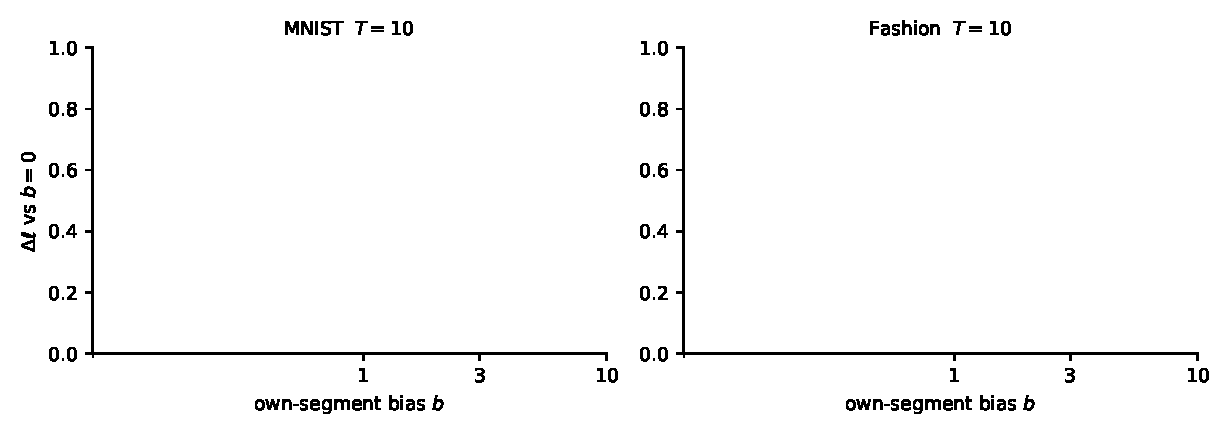
\includegraphics[width=\linewidth]{fig_dose3.pdf}
\caption{Dose--response of the own-segment bias across the three
configurations ($T{=}10$, paired means vs.\ each configuration's own
$b{=}0$). The bare MLP (blue) shows the S1 dose--response; GN-MLP
(orange) collapses to a fifth of it; ConvADNet (green) to noise.}
\label{fig:dose3}
\end{figure}

\begin{table}[t]
\centering\small
\caption{ConvADNet dose--response, paired vs.\ $b{=}0$ ($n{=}10$;
$^{*}$: $|t|>2$). Pre-registered G1 requires $\ge 15/20$ cells with
$\Delta\ell^{*}$; observed $4/12$ (no saturated cells).}
\label{tab:convdose}
\begin{tabular}{llrrr}
\toprule
cell & arm ($b$) & $\Delta\ell$ & $\Delta$avg & $\Delta$BWT \\
\midrule
MNIST $T{=}10$ & $1$ & $+0.17$ & $-1.64$ & $-2.02$ \\
MNIST $T{=}10$ & $3$ & $+0.30$ & $-0.99$ & $-1.43$ \\
MNIST $T{=}10$ & $10$ & $+0.07$ & $-0.84$ & $-1.01$ \\
Fashion $T{=}10$ & $1$ & $-0.06$ & $+0.22$ & $+0.31$ \\
Fashion $T{=}10$ & $3$ & $+0.02$ & $-0.89$ & $-1.01$ \\
Fashion $T{=}10$ & $10$ & $+0.36$ & $-2.29^{*}$ & $-2.95^{*}$ \\
MNIST $T{=}20$ & $1$ & $+0.63$ & $-0.24$ & $-0.92$ \\
MNIST $T{=}20$ & $3$ & $+1.46^{*}$ & $-0.26$ & $-1.81$ \\
MNIST $T{=}20$ & $10$ & $+1.28$ & $+0.30$ & $-1.04$ \\
Fashion $T{=}20$ & $1$ & $+0.31^{*}$ & $+0.66$ & $+0.36$ \\
Fashion $T{=}20$ & $3$ & $+0.29^{*}$ & $-0.51$ & $-0.84$ \\
Fashion $T{=}20$ & $10$ & $+0.31^{*}$ & $-0.87$ & $-1.24$ \\
\bottomrule
\end{tabular}
\end{table}

\subsection{G2 fails with a clean cause: zero mortality}
\label{sec:zeromort}

The dominant-segment instrument reads identically zero artifact:
naive share $=$ active share $=$ chance $= 1/T$ in every cell
(Table~\ref{tab:three}, column ``dead''). The cause is visible in the
per-phase instrumentation: ConvADNet's dead-gate fraction is
\emph{exactly $0.000$ in every phase of every run}, against the bare
MLP's $0.572$ \cite{zhou2026delpS1}. GroupNorm's affine output keeps
$|u| > 0$; there are no argmax ties over dead gates because there are
no dead gates (Fig.~\ref{fig:mortality}).

A measurement caveat we state explicitly: the two configurations
report mortality under \emph{different} zero-conditions. The MLP
instrument (inherited unchanged from S1) marks a neuron dead if its
post-kWTA activity is never positive across the usage window ---
mortality there means ``never wins the top-$k$ competition''. The
conv instrument marks a neuron dead if its gate row is identically
zero. Both are the natural operationalizations in their families,
but they are not the same statistic, and the conv family's
post-kWTA ``never wins'' rate was not measured. What the comparison
supports is therefore the narrower claim we make: the S1
\emph{artifact mechanism} (argmax ties over exactly-zero gates) has
no substrate on the conv configuration --- its precondition
(numerically zero gates) never occurs. The artifact is thus
\textbf{architecture-bound, not instrument-bound}: the same reading
instrument that S1 showed contaminated reads clean here, for reasons
that have nothing to do with the instrument.

\begin{figure}[t]
\centering
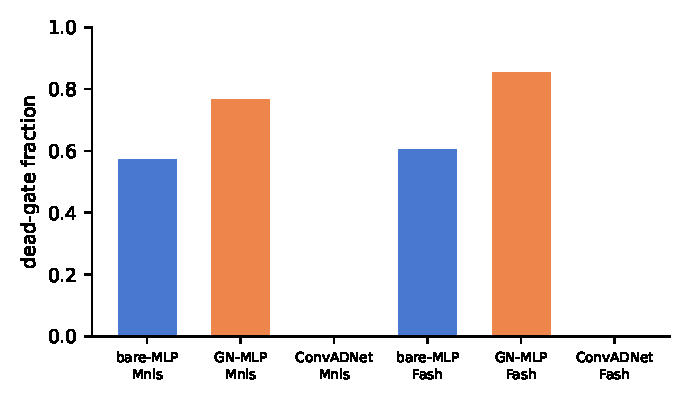
\includegraphics[width=0.72\linewidth]{fig_mortality.pdf}
\caption{Dead-gate fraction at $b{=}0$ across configurations and
datasets ($T{=}10$, mean over phases and seeds). Conv+GroupNorm
mortality is exactly zero; GroupNorm inserted into the MLP
\emph{raises} mortality. Mortality is a property of the architecture,
not of the intervention.}
\label{fig:mortality}
\end{figure}

\subsection{The conv baseline itself}

ConvADNet's unbiased baseline learns more and forgets more than the
MLP's: $\ell_0$ $84.1$/$75.3$ (vs.\ $74.3$/$56.8$) but
$\mathrm{BWT}_0$ $-50.4$/$-32.8$ (vs.\ $-11.6$/$-16.2$) at $T{=}10$.
The protection strength $\lambda{=}1000$, calibrated for the MLP's
parameter scale, does not carry over --- itself a transfer finding we
report rather than tune away (see Sec.~\ref{sec:discussion}).

% =====================================================================
\section{GN-MLP: the dying-gate hypothesis, tested and rejected}
\label{sec:gnmlp}

The natural reading of Sec.~\ref{sec:conv} is: the repair worked in
S1 because it revived dying gates, and conv gates do not die. This
``dying-gate hypothesis'' makes a sharp same-architecture prediction:
insert a normalization layer into the MLP (features $t =
\mathrm{GN}(\mathrm{ff}(x))$, the \emph{only} delta; $80$ runs,
seeds $0$--$9$, $b \in \{0,1,3,10\}$, both datasets, $T{=}10$) ---
mortality should fall and the repair should weaken accordingly.

The prediction fails in both halves (Table~\ref{tab:three}, middle
rows). Mortality \emph{rises} ($0.765$/$0.855$ vs.\ bare's
$0.572$/$0.603$), for a reason the architecture makes plain:
GroupNorm rescales the features $t$ symmetrically about zero, and the
kWTA competition keeps the $64$ \emph{largest} values of $t \odot
\sigma(d)$ --- so every neuron whose normalized feature is
predominantly negative can never enter the top-$k$ and counts as
dead under the usage instrument. GroupNorm does not touch the gate
zero-set $u$; it manufactures post-kWTA death through the feature
sign structure instead. Meanwhile the repair gain \emph{collapses
anyway}: to
$+0.57$ (retention $17\%$ of the bare-MLP gain) on MNIST and $+0.36$
($26\%$) on Fashion. And final accuracy reverses on both datasets
($\Delta\mathrm{avg} = -3.88$, $t{=}-5.3$; $-6.55$, $t{=}-4.4$).

Mortality and gain are therefore \textbf{decoupled}: one configuration
(GN-MLP) has the highest mortality and the least gain; another
(ConvADNet) has zero mortality and no gain; the bare MLP has middle
mortality and full gain. Whatever the repair feeds on, it is not gate
death per se.

\begin{table}[t]
\centering\small
\caption{The three configurations at $T{=}10$ ($n{=}10$; paired
vs.\ each configuration's own $b{=}0$). ``dead'' = mean dead-gate
fraction; ``HR$_\ell$'' = $100 - \ell_0$. The repair's
$\Delta\ell$ tracks baseline weakness, not mortality.}
\label{tab:three}
\begin{tabular}{llrrrrr}
\toprule
dataset & config & $\ell_0$ & HR$_\ell$ & dead &
$\Delta\ell_{b=10}$ & $\Delta\mathrm{avg}_{b=10}$ \\
\midrule
MNIST & bare-MLP & $74.3$ & $25.7$ & $0.572$ &
$+3.32^{*}$ & $+4.80^{*}$ \\
MNIST & GN-MLP & $93.5$ & $6.5$ & $\mathbf{0.765}$ &
$+0.57^{*}$ & $-3.88^{*}$ \\
MNIST & ConvADNet & $84.1$ & $15.9$ & $\mathbf{0.000}$ &
$+0.07$ & $-0.84$ \\
\midrule
Fashion & bare-MLP & $56.8$ & $43.2$ & $0.603$ &
$+1.39^{*}$ & $+0.69$ \\
Fashion & GN-MLP & $79.3$ & $20.7$ & $\mathbf{0.855}$ &
$+0.36^{*}$ & $-6.55^{*}$ \\
Fashion & ConvADNet & $75.3$ & $24.7$ & $\mathbf{0.000}$ &
$+0.36$ & $-2.29^{*}$ \\
\bottomrule
\end{tabular}
\end{table}

% =====================================================================
\section{What actually tracks the gain}
\label{sec:whattracks}

If not mortality, what? Table~\ref{tab:three} orders the six cells by
$\Delta\ell_{b=10}$: the bare MLPs lead on both datasets, the
strong-baseline configurations trail, and within MNIST the ordering
matches the unbiased baseline's learning-term weakness exactly
($\ell_0$ $74.3 \to 84.1 \to 93.5$ versus gain $+3.32 \to +0.07 \to
+0.57$; Fig.~\ref{fig:headroom}). We call this loose regularity
\emph{repair headroom}: the
bias can only buy learning-term room that the unbiased baseline
leaves open.

\begin{figure}[t]
\centering
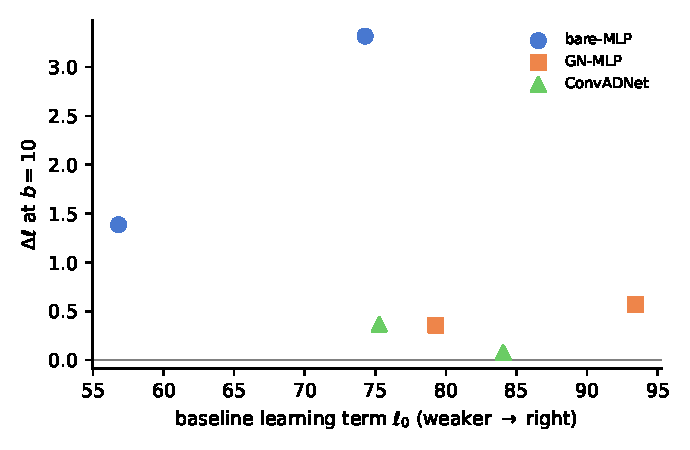
\includegraphics[width=0.72\linewidth]{fig_headroom.pdf}
\caption{Repair gain at $b{=}10$ against the unbiased baseline's
learning term. The qualitative regularity (weak baseline, larger
gain) holds within MNIST and Fashion separately, but a quantitative
law fails: ConvADNet-Fashion has $24.7$ points of $\ell$-headroom and
no significant gain. Headroom is necessary-looking, not sufficient.}
\label{fig:headroom}
\end{figure}

We stress what the data do \emph{not} support. A quantitative
headroom law fails: across the six configuration$\times$dataset
cells the Pearson correlation between HR$_\ell$ and $\Delta\ell$ is
$r = 0.38$ (cell means; pooled over per-seed differences, using each
cell's mean HR$_\ell$, $r = 0.27$; using each seed's own
$100-\ell_0$ gives $r = 0.31$), and the
 clearest counterexample is ConvADNet on Fashion --- $24.7$ points of
$\ell$-headroom, gain $+0.36$ ($t{=}1.4$, not significant). Headroom
is thus \textbf{necessary-looking but not sufficient}: a strong
baseline forecloses the repair (GN-MLP), but an open baseline does
not guarantee it (convolution adds an independent obstacle ---
plausibly the routing prior interacting with distributed conv
features, a question we leave open).

What is uniform across both strong-feature configurations is the
\emph{sign structure}: $\Delta\ell \ge 0$ (small) while
$\Delta\mathrm{avg} < 0$ (significant in $3/4$ cells;
Fig.~\ref{fig:tradeoff}). The repair
never destroys the learning term, but on strong backbones it buys
that term by trading retention --- exactly the trade S1's identity
decomposition predicts, sharpened into a reversal once the learning
side has no room left to absorb the cost.

\begin{figure}[t]
\centering
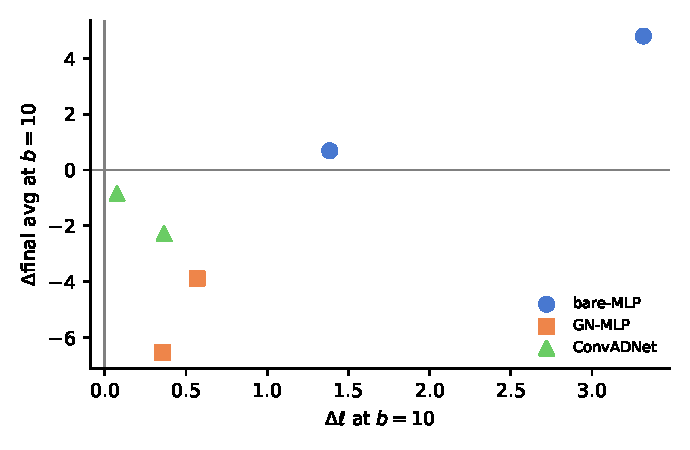
\includegraphics[width=0.72\linewidth]{fig_tradeoff.pdf}
\caption{What the bias buys and what it charges
($T{=}10$, $b{=}10$, paired means). The bare MLP sits in the
gain--gain quadrant; every strong-feature cell falls in the
learning-vs-retention trade quadrant, with final accuracy
significantly negative in $3/4$.}
\label{fig:tradeoff}
\end{figure}

% =====================================================================
\section{Discussion and boundary conditions}
\label{sec:discussion}

\paragraph{For practitioners.} An own-segment bias is cheap,
architecture-agnostic, and --- on weak baselines with hard routing ---
effective \cite{zhou2026delpS1}. This paper draws its boundary:
\begin{itemize}
\item \textbf{Audit mortality before trusting any dominant-segment
statistic.} The S1 artifact appears iff gates die; conv+GN mortality
is zero and the statistic reads clean. One probe (an untrained-pass
share, or the dead-gate fraction) is enough to know which regime you
are in.
\item \textbf{Audit baseline strength before deploying the repair.}
If the unbiased baseline's learning term is already near its ceiling,
the bias will not buy learning --- but will still charge retention
($\Delta\mathrm{avg} \le -2.3$ on every strong-feature cell,
significant in $3/4$).
\item \textbf{Protection strength does not transfer.} $\lambda$
calibrated on one parameter scale left the conv baseline with
$2$--$4.4\times$ the MLP's forgetting. Any cross-architecture
comparison of protection methods must re-calibrate or report the
uncalibrated gap explicitly.
\end{itemize}

\paragraph{For the S1 story.} The companion paper's chain survives
intact on its home architecture, and this paper sharpens its
mechanism claim: the repair was never a routing \emph{prior} in the
strong sense (S1's task-relevance probe already showed
zero-relevance tasks are untouched); it is a structured capacity
intervention whose raw material --- weak-baseline, dying-gate
networks --- is architecture-dependent. ``Structured capacity with an
architecture-bound supply.''

\paragraph{Threats to validity.} (i) The conv $\lambda$ was not
re-calibrated; a per-architecture sweep might restore some repair
effect, though the GN-MLP control --- where the MLP-calibrated
$\lambda$ \emph{is} correct --- shows the same collapse, so
mis-calibration is not the whole story. (ii) One conv topology; the
zero-mortality finding is a property of GroupNorm's affine output and
should replicate across conv trunks, but transformer backbones with
routing modules remain untested. (iii) Six configuration$\times$dataset
cells bound how strongly any cross-configuration regularity can be
asserted; we deliberately report the failed quantitative version
(Sec.~\ref{sec:whattracks}) rather than promoting the qualitative one
beyond its evidence.

% =====================================================================
\section{Conclusion}

Two pre-registered transfer attempts, $240$ runs in total, both
failed --- and the failures triangulate the mechanism. The
convolutionary active-dendrite network has no dead gates, no
dominant-segment artifact, and no repair; the GroupNorm control has
\emph{more} dead gates and \emph{less} repair. Gate death is neither
necessary nor sufficient for the own-segment bias to work. What the
repair needs is a weak baseline with learning-term room to buy; what
it always charges is retention, and on strong-feature backbones ---
where nothing else is for sale --- that is all it buys. Repairs of
this family should be deployed with a mortality probe in one hand and
a baseline audit in the other.

\section*{Data and code}

All runs, pre-registrations (written before data collection), and
analysis scripts are in the project repository:
\url{https://github.com/zhouranxi/delp-anchor-budget}
(S3\_CNN, S3b\_E4 experiment series).

\bibliographystyle{elsarticle-num}
\bibliography{refs}

\end{document}
